% Chapter Template

\chapter{Interspecific shared collective decision-making in two forensically important species} % Main chapter title

\label{Chapter4} % Change X to a consecutive number; for referencing this chapter elsewhere, use \ref{ChapterX}

\lhead{Chapitre 4. \emph{Interspecific shared collective decision-making in two forensically important species}} % Change X to a consecutive number; this is for the header on each page - perhaps a shortened title

Julien \textsc{Boulay}\up{a,b}, Jean-Louis \textsc{Deneubourg}\up{b},  Valéry \textsc{Hédouin}\up{a} and \\ Damien \textsc{Charabidzé}\up{a}

\up{a} Univ. Lille, CHU Lille, EA 7367 - UTML - Unité de Taphonomie Médico-Légale, Lille, France\\
\up{b} Université Libre de Bruxelles, Unit of Social Ecology, Brussels, Belgium\\




Article resoumis à \emph{Proceedings of the Royal Society of London B}.


\cleardoublepage
%----------------------------------------------------------------------------------------
%	SECTION 1
%----------------------------------------------------------------------------------------
	\section{Abstract}
To date, the study of collective behaviour has mainly focused on intraspecific situations. Collective decision-making of mixed-species groups, involving interspecific aggregation-segregation, have received little attention. The study of such groups provides the opportunity to place the evolution of sociality in ecological and interspecific cooperation contexts. Here, we show that, in both conspecific and heterospecific groups, two gregarious larvae species were able to make a clear collective decision for one food spot. We observed similar dynamics between the two studied species: in both species, the choice was made within a few minutes and persisted throughout the experiment period. The monitoring of a focal individual within a group showed that these aggregations were governed by attractive and retentive effects of the group. The similarity observed between the conspecific and heterospecific groups suggested the existence of shared aggregation signals. These results can be characterized in larvae by a positive correlation between group size and heat generation; in the present study, the group size was found to have a stronger influence than the species of necrophagous larvae. This study provides the first experimental evidence of the dynamics of collective decisions-making in mixed-species groups of invertebrates, contributing to our understanding of the cooperation-competition phenomenon in animal social groups.

\textit{Keywords:} amplification – binary choice – gregariousness – marking – mixed-species group – tracking 

\clearpage

%----------------------------------------------------------------------------------------
%	SECTION 2
%----------------------------------------------------------------------------------------
	\section{Background}
To date, the study of collective behaviour has mainly focused on species with a high level of sociality \cite{costa_other_2006}. As a result, species with a lower level of social organization, such as those that exhibit gregariousness, have comparatively received little attention \cite{costa_other_2006}. However, the understanding of the key factors that permit the emergence of a collective decision in a large group composed of simple individuals (having a limited knowledge of their close environment) is fundamental to deciphering the evolution of sociality. Gregarism, which is observed in many species from mammals to unicellular species \citep{costa_other_2006,krause_living_2002,sumpter_collective_2009,parrish_complexity_1999}, can be defined as a gathering (i.e., an inter-attraction) of individuals independent of reproduction. Several insect species are gregarious at the larval instar and/or adult level \citep{costa_other_2006,jeanson_key_2012}. To find, form, stabilize or split aggregates, insects use various signals or cues (e.g., chemical, tactile and visual) \citep{costa_other_2006,krause_living_2002,sumpter_collective_2009,camazine_self-organization_2001}. In this context, the self-organization theory, independent of the nature of the interaction, has been successfully used to explain how simple interactions between individuals having only local information can generate a diversity of complex patterns at the collective level \citep{camazine_self-organization_2001,deneubourg_dynamics_2002,deneubourg_collective_1989}. It has been shown that consensus choices, called 'collective decisions' \citep{jeanson_key_2012,conradt_consensus_2005}, are made by various conspecific groups of insect species; a review on this topic was published by \citet{jeanson_key_2012}. Mixed-species groups are found in a large range of taxons from mammals \cite{stensland_mixed_2003} to birds \cite{farine_collective_2014}. Such groups offer identical benefits to those achieved by non-mixed groups, such as a protection from predators and efficient foraging behaviour \cite{costa_other_2006}. The existence of heterospecific groups raises the question of how sociality evolved in animals \citep{costa_other_2006,wilson_insect_1971}. ]. It also allows a discussion of new perspectives for livestock management to improve breeding conditions of species living together \cite{anderson_managing_2012}. Moreover, the existence of such groups suggests that similar, or close, aggregation cues are used by individuals regardless of species (cross-species recognition). Fewer studies have investigated heterospecific groups \cite{stensland_mixed_2003,farine_mixed-species_2014,diamond_mixed-species_1981}, particularly with regard to their collective decision-making abilities \cite{farine_collective_2014}. Some results regarding heterospecific associations in Diptera species have been reported in the context of species coexistence and competition \cite{dos_reis_larval_1999}, but no study has yet investigated the collective decisions of a mixed group from a quantitative point of view.\\
Aggregations of Diptera larvae, including heterospecific groups, have been extensively reported in the forensic entomology literature but remain poorly understood \citep{rivers_physiological_2011,charabidze_larval-mass_2011,boulay_evidence_2013,heaton_quantifying_2014}. Recently, \citet{boulay_evidence_2013} demonstrated that these aggregations are active and associated with chemical cues given by larvae of the blow fly \textit{Lucilia sericata}. \citet{rivers_physiological_2011} identified the benefits of maggot masses, such as heat generation, called the ‘larval-mass effect’ \cite{charabidze_larval-mass_2011}, and cooperation for the assimilation of food and digestion (increasing the local quantity of enzymes \cite{wilson_impacts_2015}). Regarding these benefits, aggregation behaviour facilitates cooperation and therefore permits an acceleration of larval development and increases in larval survival and carrion decomposition. Such benefits can be regarded as a source of the Allee effect \citep{courchamp_allee_2008,wilson_impacts_2015}.

The present study aimed to highlight the communal collective decision-making process of mixed-species groups leading to the choice of one food-spot. This study used \textit{L. sericata} and \textit{Calliphora vomitoria} larvae, two key species in forensic entomology that often feed simultaneously on carrion \cite{amendt_forensic_2004}. For this purpose, binary choice tests were performed between two identical food spots. The binary choice test has been used in several studies to highlight collective decision-making (see review in \citet{jeanson_key_2012}) and is also relevant to study necrophagous larvae (supplementary material, Figure \ref{fig:cochon}). Indeed, these species are often observed on symmetric cadavers, such as large mammals or rodents, which offer several identical spots for larvae to form groups on.
    
%----------------------------------------------------------------------------------------
%	SECTION 3
%----------------------------------------------------------------------------------------
	\section{Methods}
		\subsection{Insect rearing}
Larvae (maggots) were obtained from colonies bred at the Forensic Institute of Lille (Nord, France). Adult \textit{Lucilia sericata} and \textit{Calliphora vomitoria} were reared in separate cages at ambient temperature (20 $\pm$2\up{o}C) under daylight (12:12 h). The flies were fed caster sugar and water ad libitum. Upon the emergence of adult flies (day 0), minced beef liver was added for seven days (i.e., until day 7) to provide the protein required for vitellogenesis. After five days with no food, liver was again provided for use as an oviposition medium (day 12). After 24 h (day 13), eggs of \textit{L. sericata} and \textit{C. vomitoria} were separately placed on the breeding substrate (100 g of fresh minced beef liver). Larvae of \textit{L. sericata} were bred at 17$\pm$0.5\up{o}C, and after 5 to 6 days (day 18-19), young 3\up{rd}-instar larvae (10 $\pm$2mm in length) were sampled for the experiments \cite{grassberger_effect_2001}. Larvae of \textit{C. vomitoria} were bred at 20$\pm$0.5\up{o}C, and after 11 to 12 days (days 24-25), young 3rd-instar larvae (11 $\pm$2mm in length) were sampled for the experiments \cite{ames_low_2003}. The number of larvae used in each experiment (40) was sufficiently low to avoid autogenous heat emission (i.e., the larval-mass effect) \citep{charabidze_larval-mass_2011,heaton_quantifying_2014}.
    

		\subsection{Experimental setup}
The experimental arena consisted of an 18.5-cm-diameter Pyrex\up{®} glass Petri dish. The dish was filled to a height of 1 cm with agar-agar (7 g/250 ml) with two diametrically opposed food spots (5.5 cm in diameter), each situated 2 cm from the edge of the arena. These spots were designated as the west and east spots. Each spot consisted of a solution of liver (mean nutritional composition: 15.4$\%$ proteins, 7.3$\%$ carbohydrates and 4.1$\%$ fats (National Sanitary Security Agency)) and water (6 g/50 ml) mixed with agar. This food solution attracted a sufficient number of individuals and permitted clear counts of the number of individuals within each food spot, and each spot was sufficiently large to accommodate all of the larvae used in the trial (pers. obs.). Both food spots were strictly identical in size, composition and distance from the edge of the arena. The arena was placed in a climatic chamber (Firlabo) at 25$\pm$1\up{o}C and monitored by video.
	
    
		\subsection{Experimental procedure}
Before each trial, the larvae were removed from the feeding substrate, placed in wet pine-wood dust and isolated in the dark at 25$\pm$1\up{o}C for 1 h. This isolation time starved the larvae while the sawdust removed traces of food from their cuticles \cite{charabidze_discontinuous_2013}. Three conditions, including two conspecific conditions and one heterospecific condition, were tested: (1) 40 \textit{Lucilia sericata} larvae (N=30; conspecific condition), (2) 40 \textit{Calliphora vomitoria} larvae (N=30; conspecific condition) and (3) 20 \textit{L. sericata} + 20 \textit{C. vomitoria} larvae (N=30; heterospecific condition).


		\subsection{Conspecific condition and individual tracking}	
For each condition, forty larvae were randomly placed in a fresh arena in a dark room due to their high photophobic behaviour \cite{hinnemann_see_2010}. The arena was lit from below with a fluorescent neon light (8 W; Velopex) with a red ROSCO\up{TM} filter (ref. Roscolux $\sharp$19 Fire). This filter changed the spectrum of light by transmitting predominantly red wavelengths, which are not perceived by larvae \cite{hinnemann_see_2010}. The aggregation process was video-recorded over 60 min using a Bosch Dinion LTC0355 camera. The number of larvae in each of the three zones (the two spots and the area outside of the two spots) was counted visually at 1-min intervals. To be considered located outside of a spot, the individual had to have its entire bodies outside of the spot.\\
In each trial, a single larva was tracked throughout the 60-min trial period. To facilitate tracking, the selected focal individual was 1 mm longer than the other 39 individuals. Videos were down-sampled every 5 s (720 frames per video), and the position of the tracked larva was determined using Avimeca 2.7 freeware. The mid-point of the larval body was used for tracking. For the individual tracking analysis, we virtually enlarged the radius of each spot based on our tracking method (mid-point of the body) and the mean size of the individuals (10 $\pm$2mm). Such enlargement was set to 1 cm, corresponding to one larval body length increasing the radius from 2.25 cm to 3.25 cm.


		\subsection{Heterospecific condition}
Because the larvae of the two species are very similar in appearance, we marked the individuals according to their species to distinguish them during the heterospecific experiment. Twenty individuals of one species were marked using Lumicyano\up{TM} (Crime Scene Technology), a cyanoacrylate fluorescent glue that reacts to ultraviolet light \cite{prete_lumicyano:_2013}. The marking consisted of a small spot (1 mm\up{2}; Figure \ref{fig:lumi}) of Lumicyano\up{TM} placed on the anterior region of the larva’s dorsal surface. We used this glue to create UV-bright spots, thereby marking individuals according to species \cite{prete_lumicyano:_2013}. Lumicyano\up{TM} is very powerful and robust, dries quickly (2-3 s) and is available in several colours. These characteristics are useful for marking larvae with viscous cuticles and fast-moving species on which marking must be performed rapidly. Maggots are burrowing insects: they secrete a fat cuticular compound, crawl into cadavers and are often partially covered with decomposed flesh. In large masses composed of thousands of individuals, maggots move rapidly in a permanent turnover, creating high scramble competition \cite{rivers_physiological_2011}. These traits make it difficult or impossible to use the standard marking techniques for identifying and tracking insects \cite{hagler_methods_2001}. In a recent study, \citet{rosati_investigating_2015} successfully fed larvae with fluorescent fingerprint powders to obtain marked blowfly larvae. In the present study, in which the larvae were observed under dark and non-stress conditions, we developed an innovative, non-invasive marking method that allowed the tracking of larvae under UV light using a cyanoacrylate glue (Lumicyano\up{TM} \cite{prete_lumicyano:_2013}). Using this technique, we provide the first demonstration and quantification of a mixed-species aggregation with collective interspecific decision-making.\\
In contrast to the technique used by \citet{rosati_investigating_2015}, our method can be used with all blowfly larval instars and with other arthropod species (e.g., phytophagous taxa), and researchers can draw patterns or numbers to precisely identify individuals. This technique can also be used on several individuals simultaneously. Previous observations showed that the marking did not affect larval movement (test of aggregation with twenty marked individuals and twenty unmarked individuals in a monospecific condition; supplementary material, Figure \ref{fig:species}), and the marking was alternated between the two species before each trial. The arena was lit by two ultraviolet lights (2x15 W; Omnilux) because ultraviolet wavelengths are not perceived by larvae \cite{hinnemann_see_2010}. The aggregation process was video-recorded for 60 min using a 5-megapixel camera (GoPro Hero 3+\up{TM}, GoPro Enterprise). No individual tracking was performed during the heterospecific experiments due to the marking method and light conditions.

\begin{figure}[ht]
\centering
		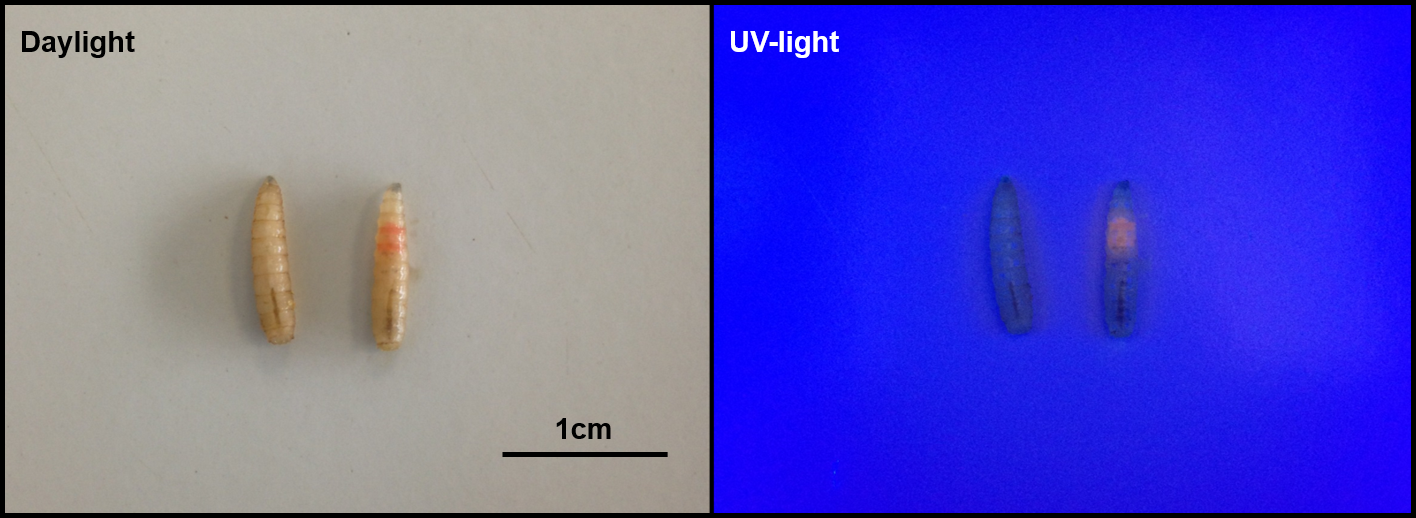
\includegraphics[width=0.8 \textwidth]{Figures/lumicyano.png}
		\rule{35em}{0.5pt}
		\caption[Lumi]{\textbf{\textit{Lucilia sericata} larvae, including non-marked larvae and larvae marked using Lumicyano\up{TM}}. For marking, a small spot of the cyanoacrylate UV-bright glue (1 mm\up{2}) was placed on the anterior part of an individual (on the larva’s crop).}
	\label{fig:lumi}
\end{figure}


		\subsection{Data analysis}
Trials resulting in an aggregation of individuals outside of either spot (denoted ‘outside trials’) were excluded from the analysis (corresponding to two trials of the \textit{L. sericata} group, four trials of the \textit{C. vomitoria} group and six trials of the heterospecific condition (mean proportion of outside trials: 13 $\pm$7$\%$). In total, 28 replicates were analysed for the \textit{L. sericata} group, 26 replicates were analysed for the \textit{C. vomitoria} group, and 24 replicates were analysed for the heterospecific group.\\
To verify that our setup was not biased for the left or right spot, we performed binomial tests. In support of the non-biased setup hypothesis, no side-related differences were observed between the two spots (west and east) during either the conspecific or heterospecific experiments (binomial tests for \textit{L. sericata}: p=0.16; for \textit{C. vomitoria}: p=0.18; for the heterospecific condition: p=0.17). Larvae did not choose one side of the arena more than the other one.\\
The spot with the largest number of individuals at the end of the experiment was designated the ‘Winner spot’, whereas the other spot was designated the ‘Loser spot’ (binomial test at t=60 min) \citep{halloy_social_2007,sempo_complex_2009}. To verify the neutrality of the setup, binomial tests were performed with the hypothesis H$_{0}$ assuming an equal distribution of individuals between the two spots (west and east). The data were tested for deviance from normality using the Kolmogorov-Smirnov test. Parametric tests were used if data normality and homogeneity of variance were observed; otherwise, corresponding non-parametric tests were used. The statistical tests were two-tailed and performed using GraphPad InStat 3.06 for Windows. All of the analyses assumed a significance level of $\alpha$ = 0.05, unless otherwise stated. For Dunn’s multiple paired comparison tests, the significance level $\alpha$ was adjusted using the Bonferroni method \cite{zar_biostatistical_2010}.


%----------------------------------------------------------------------------------------
%	SECTION 4
%----------------------------------------------------------------------------------------
	\section{Results}
		\subsection{Conspecific condition}
Of the 28 replicates performed with \textit{L. sericata}, we observed 20 replicates in which one food spot was preferentially chosen over the other at the end of the trial (binomial tests: p=0.01; supplementary material, Video S3). For \textit{C. vomitoria}, we observed 20 replicates out of 26 in which one food spot was preferentially chosen over the other (binomial tests: p=0.004; supplementary material, Video S4). On average, more than 50$\%$ of the individuals were found on the Winner spot (mean$\pm$SD; \textit{L. sericata}: 50.8$\pm$18$\%$; C. vomitoria: 57.2$\pm$14$\%$; Figure \ref{fig:choix}), whereas the Loser spot attracted less than 20$\%$ of the individuals (\textit{L. sericata}: 18.9$\pm$12$\%$; \textit{C. vomitoria}: 19$\pm$13$\%$; Figure \ref{fig:choix}). These percentages reflect a clear trend of collective choice for one spot (i.e., the Winner spot) by both species. Furthermore, the dynamics of these collective choices were similar between the two species. Each collective choice was made within 2 min of the start of the trial, with the majority of the individuals going to one spot (i.e., the Winner spot) (Wilcoxon tests at t=1 min Winner spot vs. Loser spot; \textit{L. sericata}, W=160, p=0.04;\textit{C. vomitoria}, W=189, p=0.003; Figure \ref{fig:choix}). In both conspecific conditions, these collective choices were made very rapidly and persisted throughout the trial period (Figure \ref{fig:choix}).


\begin{figure}[ht]
\centering
		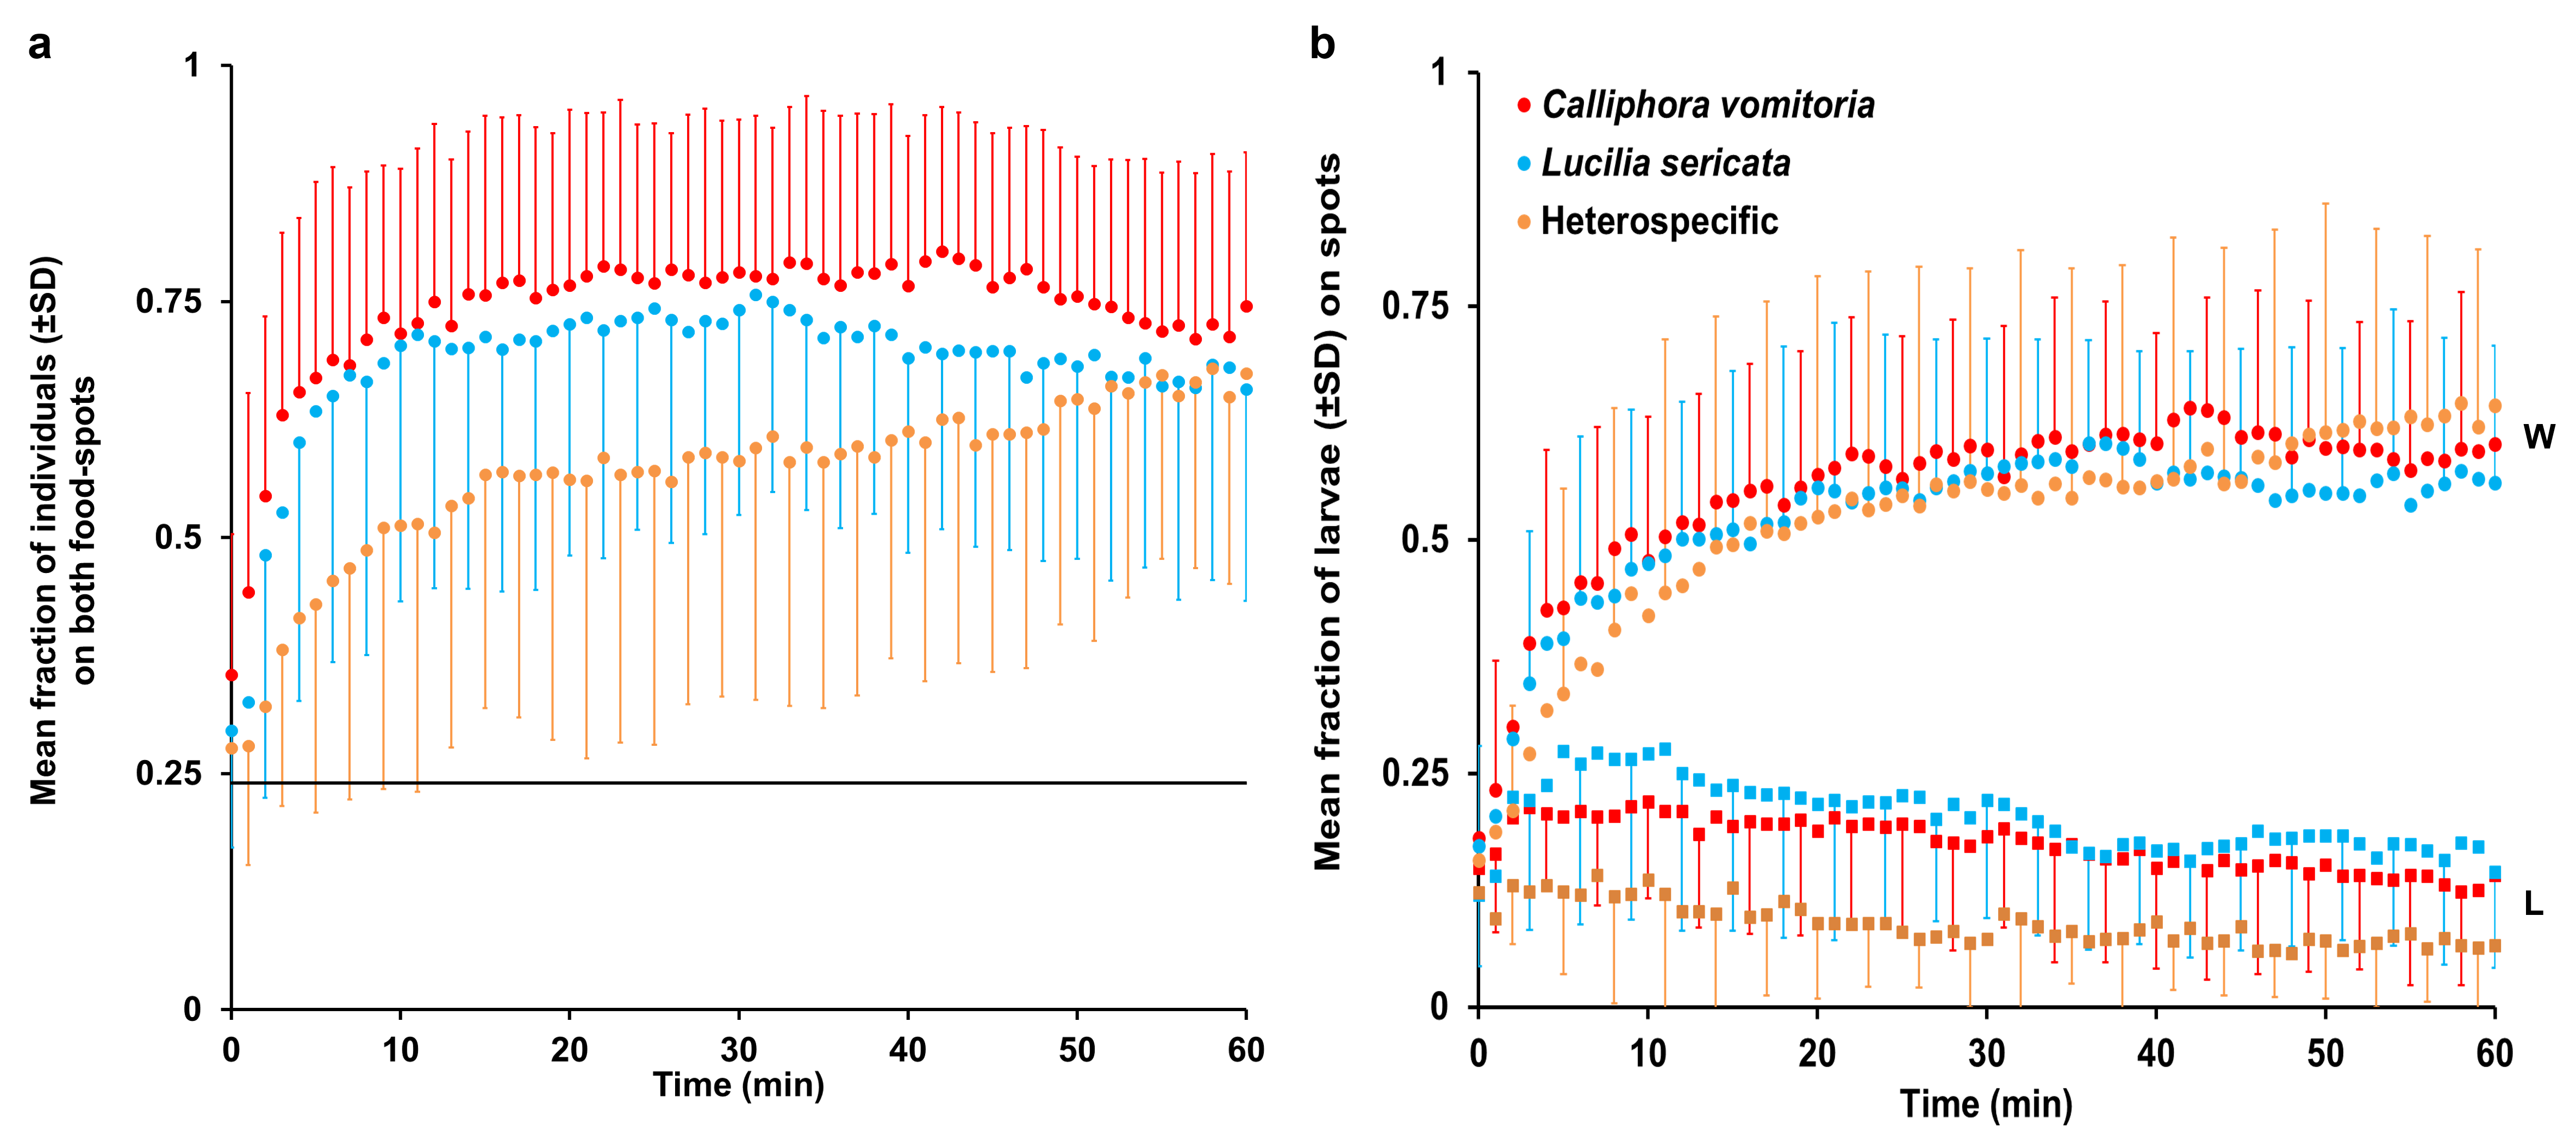
\includegraphics[width=1 \textwidth]{Figures/choix.png}
		\rule{35em}{0.5pt}
		\caption[Choix]{\textbf{Aggregation kinetics of conspecific and heterospecific groups}. \textbf{a}, Mean fraction of individuals in conspecific (\textit{Calliphora vomitoria} (red, N=26); \textit{Lucilia sericata} (blue, N=28)) and heterospecific groups (orange, N=24) on both food-spots over time. The horizontal line corresponds to a random distribution of individuals on the surface, which was calculated according to \citet{canonge_group_2011}. No differences were observed at t=0 min between a random distribution and the three observed distributions (bilateral tests: \textit{C. vomitoria}: u=1.37, p>0.05; \textit{L. sericata}: u=0.69, p>0.05; heterospecific group: u=0.42, p>0.05; $\text{u}_{\text{alpha}}$=1.96). Significant differences from a random distribution were observed 2 min after trial initiation for the \textit{L. sericata} groups, 1 min after trial initiation for the \textit{C. vomitoria} groups and 4 min after trial initiation for the heterospecific groups (using bilateral tests). The two monospecific kinetics presented no differences from t=0 min to t=60 min (Mann-Whitney tests). Multiple comparisons among the three conditions showed no significant differences from t=40 min (KW=5.12, p=0.08) to t=60 min (KW=2.48, p=0.29). Such comparisons showed that heterospecific groups aggregate more slowly than the two monospecific groups on both spots. \textbf{b}, Aggregation dynamics of 40 larvae in conspecific (\textit{C. vomitoria}, N=26; \textit{L. sericata}, N=28) and heterospecific groups (24 replicates; 20 individuals of each species). Mean fraction of individuals ($\pm$SD) found on the Winner spot (W; represented by circles) and the Loser spot (L; represented by squares). No differences were observed at t=60 min between the three conditions with respect to the Winner spot \\(KW=3.72, p=0.16) or the Loser spot (Dunn’s test, $\alpha$=0.017, p>0.05).}
	\label{fig:choix}
\end{figure}

		\subsection{Heterospecific condition}
In the 24 replicates performed with the two species together, we observed only three replicates in which no spot was preferentially chosen over the other. Of those trials yielding a clear choice of one spot, the two species chose the same Winner spot in 100$\%$ of cases (supplementary material, Video S5). The aggregation dynamics of the heterospecific groups were similar to those of the conspecific groups but required more time to join the plateau value of intraspecific groups (Figure \ref{fig:choix}). Indeed, at t=0 min, no differences were observed between the three conditions (KW=3.95, p=0.14; Figure \ref{fig:choix}). At t=2 min, the heterospecific groups were significantly different compared with the two monospecific groups (KW=14.96, p<0.001; Dunn’s test, $\alpha$=0.017, p<0.001; Figure \ref{fig:choix}). The heterospecific groups rejoined, in terms of the number of individuals, the two monospecific groups at t=40 min (KW=5.12, p=0.08), and this similarity lasted until the end of experiment (t=60 min, KW=2.48, p=0.29; Figure \ref{fig:choix}). These results show that the heterospecific groups aggregated more slowly on both spots than the two conspecific groups. The Winner spot contained more than 50$\%$ of the individuals (53.8$\pm$26$\%$; Figure \ref{fig:choix}), whereas the Loser spot attracted 8.1$\pm$7$\%$ of the larvae. On each spot, the number of larvae was balanced between the two species (e.g., Winner spot, t=30 min: \textit{L. sericata}: 10.1$\pm$5.6, \textit{C. vomitoria}: 10.1$\pm$5.5, t=0.72, p<0.001; Winner spot, t=60 min: \textit{L. sericata}: 12.0$\pm$5; \textit{C. vomitoria}: 11.5$\pm$5.1, t=15.2, p<0.001; Loser spot, t=30 min: \textit{L. sericata}: 1.4$\pm$1.6; \textit{C. vomitoria}: 1.7$\pm$1.7, t=4.3, p<0.001; Loser spot, t=60 min: \textit{L. sericata}: 1.1$\pm$1.3; \textit{C. vomitoria}: 1.9$\pm$2, t=3.7, p<0.001; supplementary material, Figure \ref{fig:species}). This result demonstrates that aggregation on the Winner spot was equally composed of both species over time, as determined based on the numbers of individuals.


		\subsection{Individual tracking}
The individual tracking of one larva during each trial was useful for understanding individual behaviour and how collective choice arises from larval displacements. The individual tracks showed that the larvae did not always remain on the Winner spot throughout the trials (Figure \ref{fig:tracking}). The larvae were highly mobile, moving back and forth on the Winner spot as well as exploring the Loser spot (Figure \ref{fig:tracking}). This observation was confirmed by analysing the mean duration of time spent on the Winner spot: larvae remained on it for only a short period of time (\textit{L. sericata}: 84.6$\pm$112 s; \textit{C. vomitoria}: 137.6$\pm$246 s; U=47308, p=0.03). However, foraging behaviour was clearly oriented toward the Winner spot; although this spot represented only 5.9$\%$ of the total test area, the mean time spent by the larvae on the Winner spot was 1616$\pm$750 s for \textit{L. sericata} and 1953.5$\pm$782 s for \textit{C. vomitoria}, representing 44$\%$ and 55$\%$ of the total experiment duration, respectively (bilateral test: u=0.63, $\text{u}_{\text{alpha}}$=1.96, p=0.49). Conversely, the larvae also remained on the Loser spot for a short period of time (\textit{L. sericata}: 46.4$\pm$76 s; \textit{C. vomitoria}: 84.4$\pm$209 s; U=11581, p=0.2). Individuals of \textit{L. sericata} spent 12$\%$ of the total experiment duration on the Loser spot (447.5$\pm$351 s), and \textit{C. vomitoria} individuals spent 15$\%$ of their time on this spot (552.8$\pm$808 s) (u=0.28, $\text{u}_{\text{alpha}}$=1.96, p=0.14). Positive relationships were observed between the time spent on the spots by the tracked individuals and the number of individuals present on the spot at this time (Figure \ref{fig:timenumb}). The larvae tended to stay longer on the Winner spot if the number of individuals already on the spot was high, suggesting a retentive effect of the group (Figures \ref{fig:timenumb} and \ref{fig:groupeffect}). Moreover, the time spent in the two other zones of the arena (Outside + Loser spot) tended to decrease as the number of larvae on the Winner spot increased (Figure \ref{fig:groupeffect}). Such results suggest the existence of an attractive effect of the group.

Additionally, the probability of returning to the Winner spot was higher than the probability of returning to the Loser spot for both species (the number of transitions from Winner-to-Winner was higher than that from Loser-to-Loser for both species; supplementary material, Figure \ref{tab:transition}). Moreover, the mean time to exit one spot and return to the same spot was shorter than that found for changing spots (supplementary material, Figure \ref{tab:transition}). These results are in agreement with the observation that larvae of the two species mostly moved near the edge of the Winner spot (Figure \ref{fig:tracking}) and reinforce the hypothesis of the existence of a retention effect of the group on the larvae (Figure \ref{fig:groupeffect}).

\begin{figure}[p]
\centering
		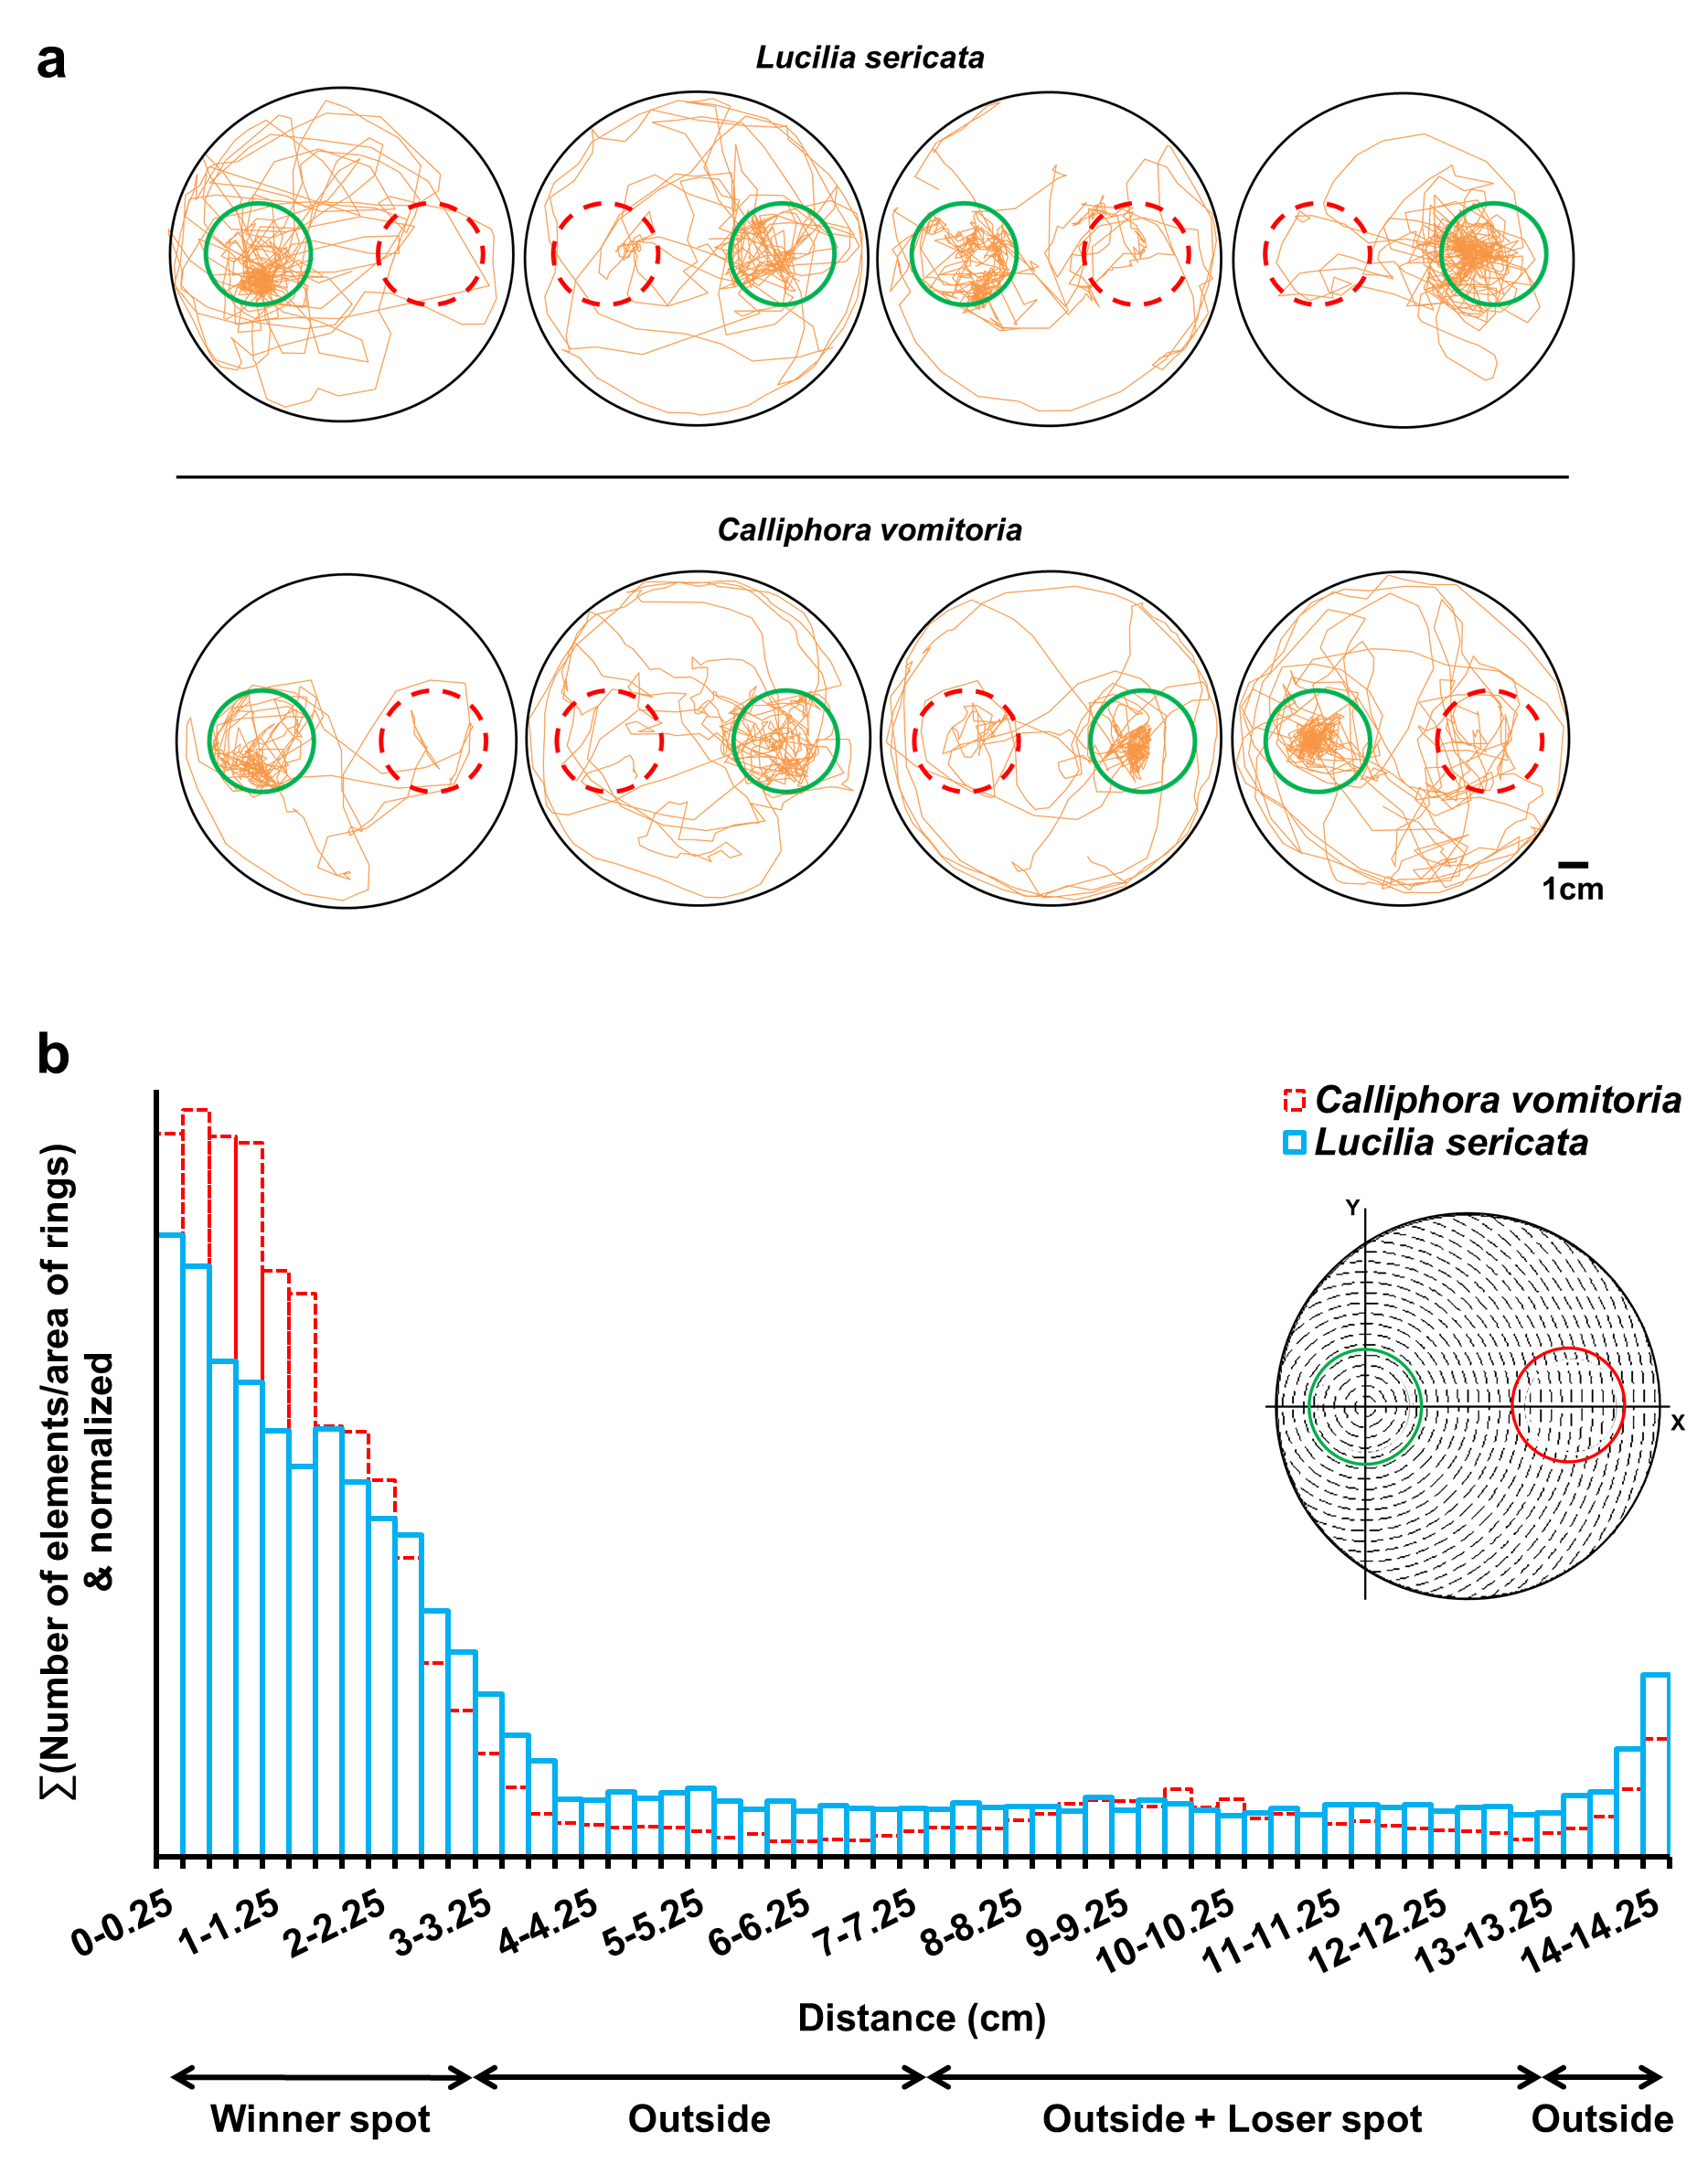
\includegraphics[width=0.8 \textwidth]{Figures/tracking.png}
		\rule{35em}{0.5pt}
		\caption[Tracking]{\textbf{Individual behaviour of larvae.} \textbf{a}, Tracks of eight larvae followed for 60 min during the conspecific experiment. The green circles represent the Winner spots, and the dotted red circles represent the Loser spots (diameter: 3.25 cm). \textbf{b}, Relative density of tracked larvae according to the distance (cm) from the centre of the Winner spot (conspecific experiments, N=20 for each species). The centre of the Winner spot was used as the reference coordinate (the Winner spot is represented by green, and the Loser spot is shown in red; diameter: 3.25 cm). The sum of the number of elements (distance to the centre of the Winner spot) divided by the ring area (see the illustration) is shown along the Y-ordinate axis.}
	\label{fig:tracking}
\end{figure}

\begin{figure}[p]
\centering
		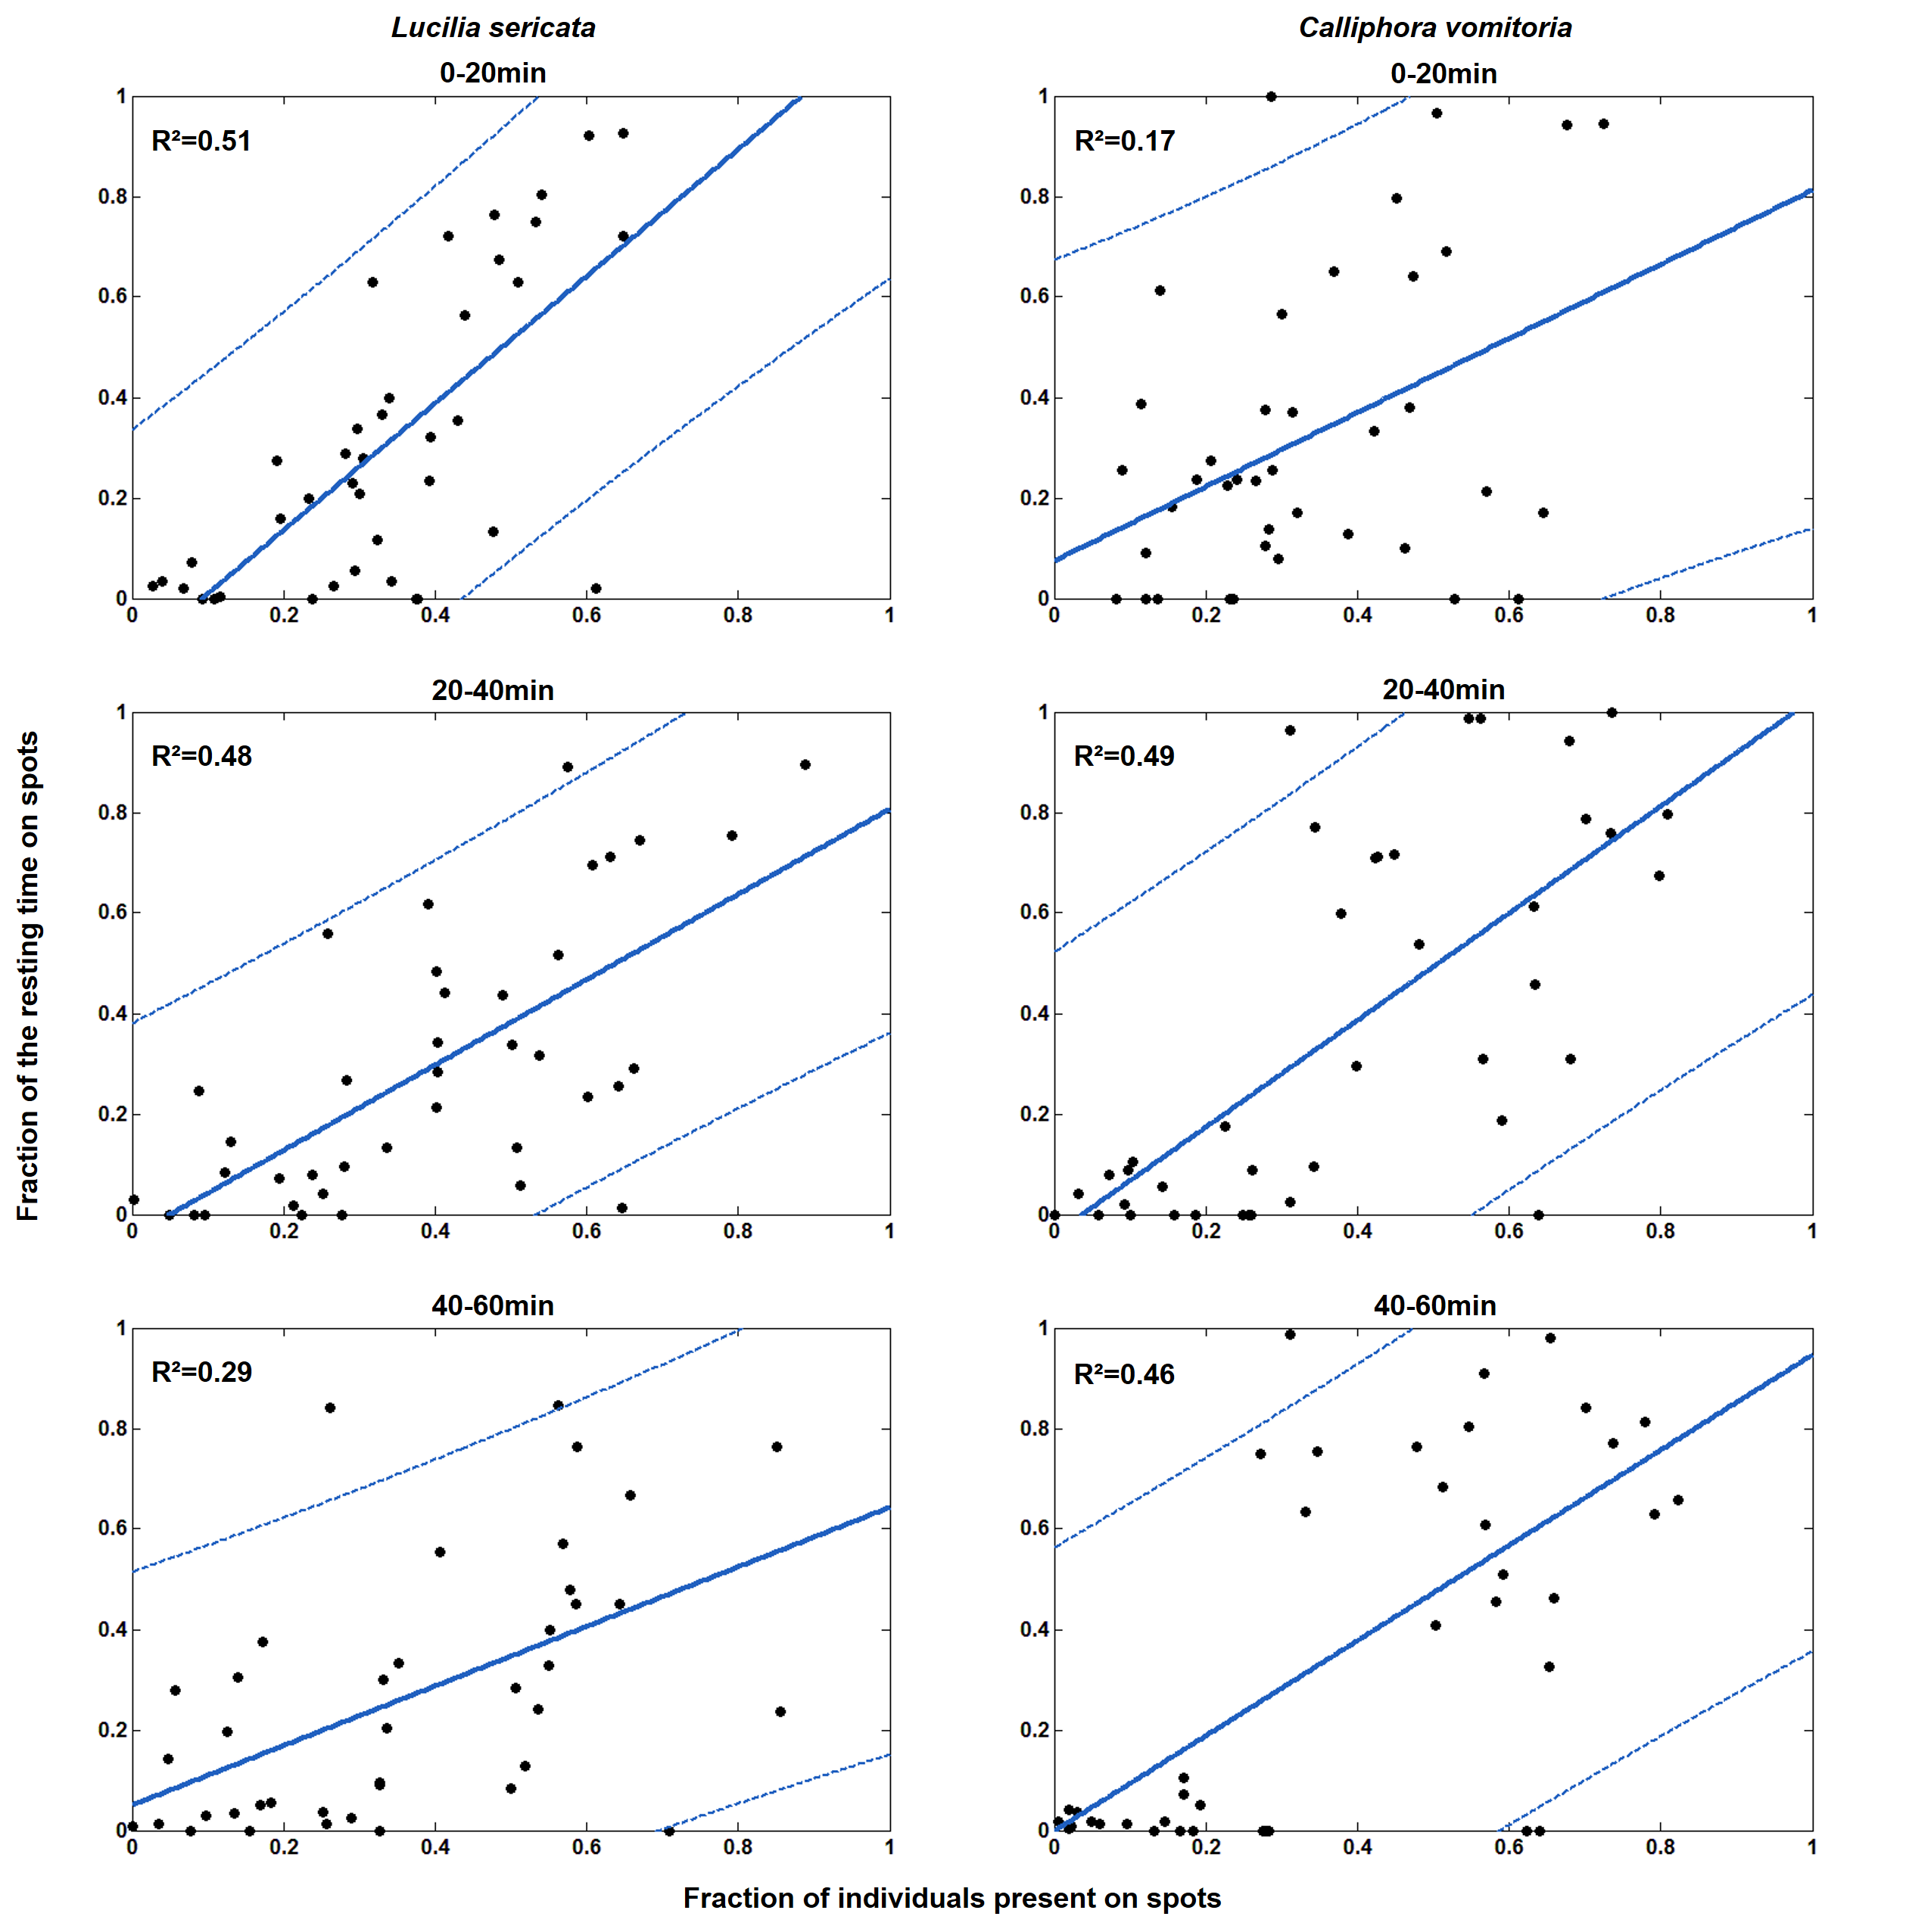
\includegraphics[width=1 \textwidth]{Figures/time_number.png}
		\rule{35em}{0.5pt}
		\caption[Timenumb]{\textbf{Time spent by tracked individuals on each spot according to the number of individuals present}. The trial duration was divided into three time periods. For each time period, the fraction of resting time on both spots (Winner and Loser) was plotted as a function of the fraction of individuals present on the corresponding spots. All of the linear regression slopes differed significantly from zero. \\The dotted lines correspond to the 95$\%$ CIs.}
	\label{fig:timenumb}
\end{figure}

\begin{figure}[p]
\centering
		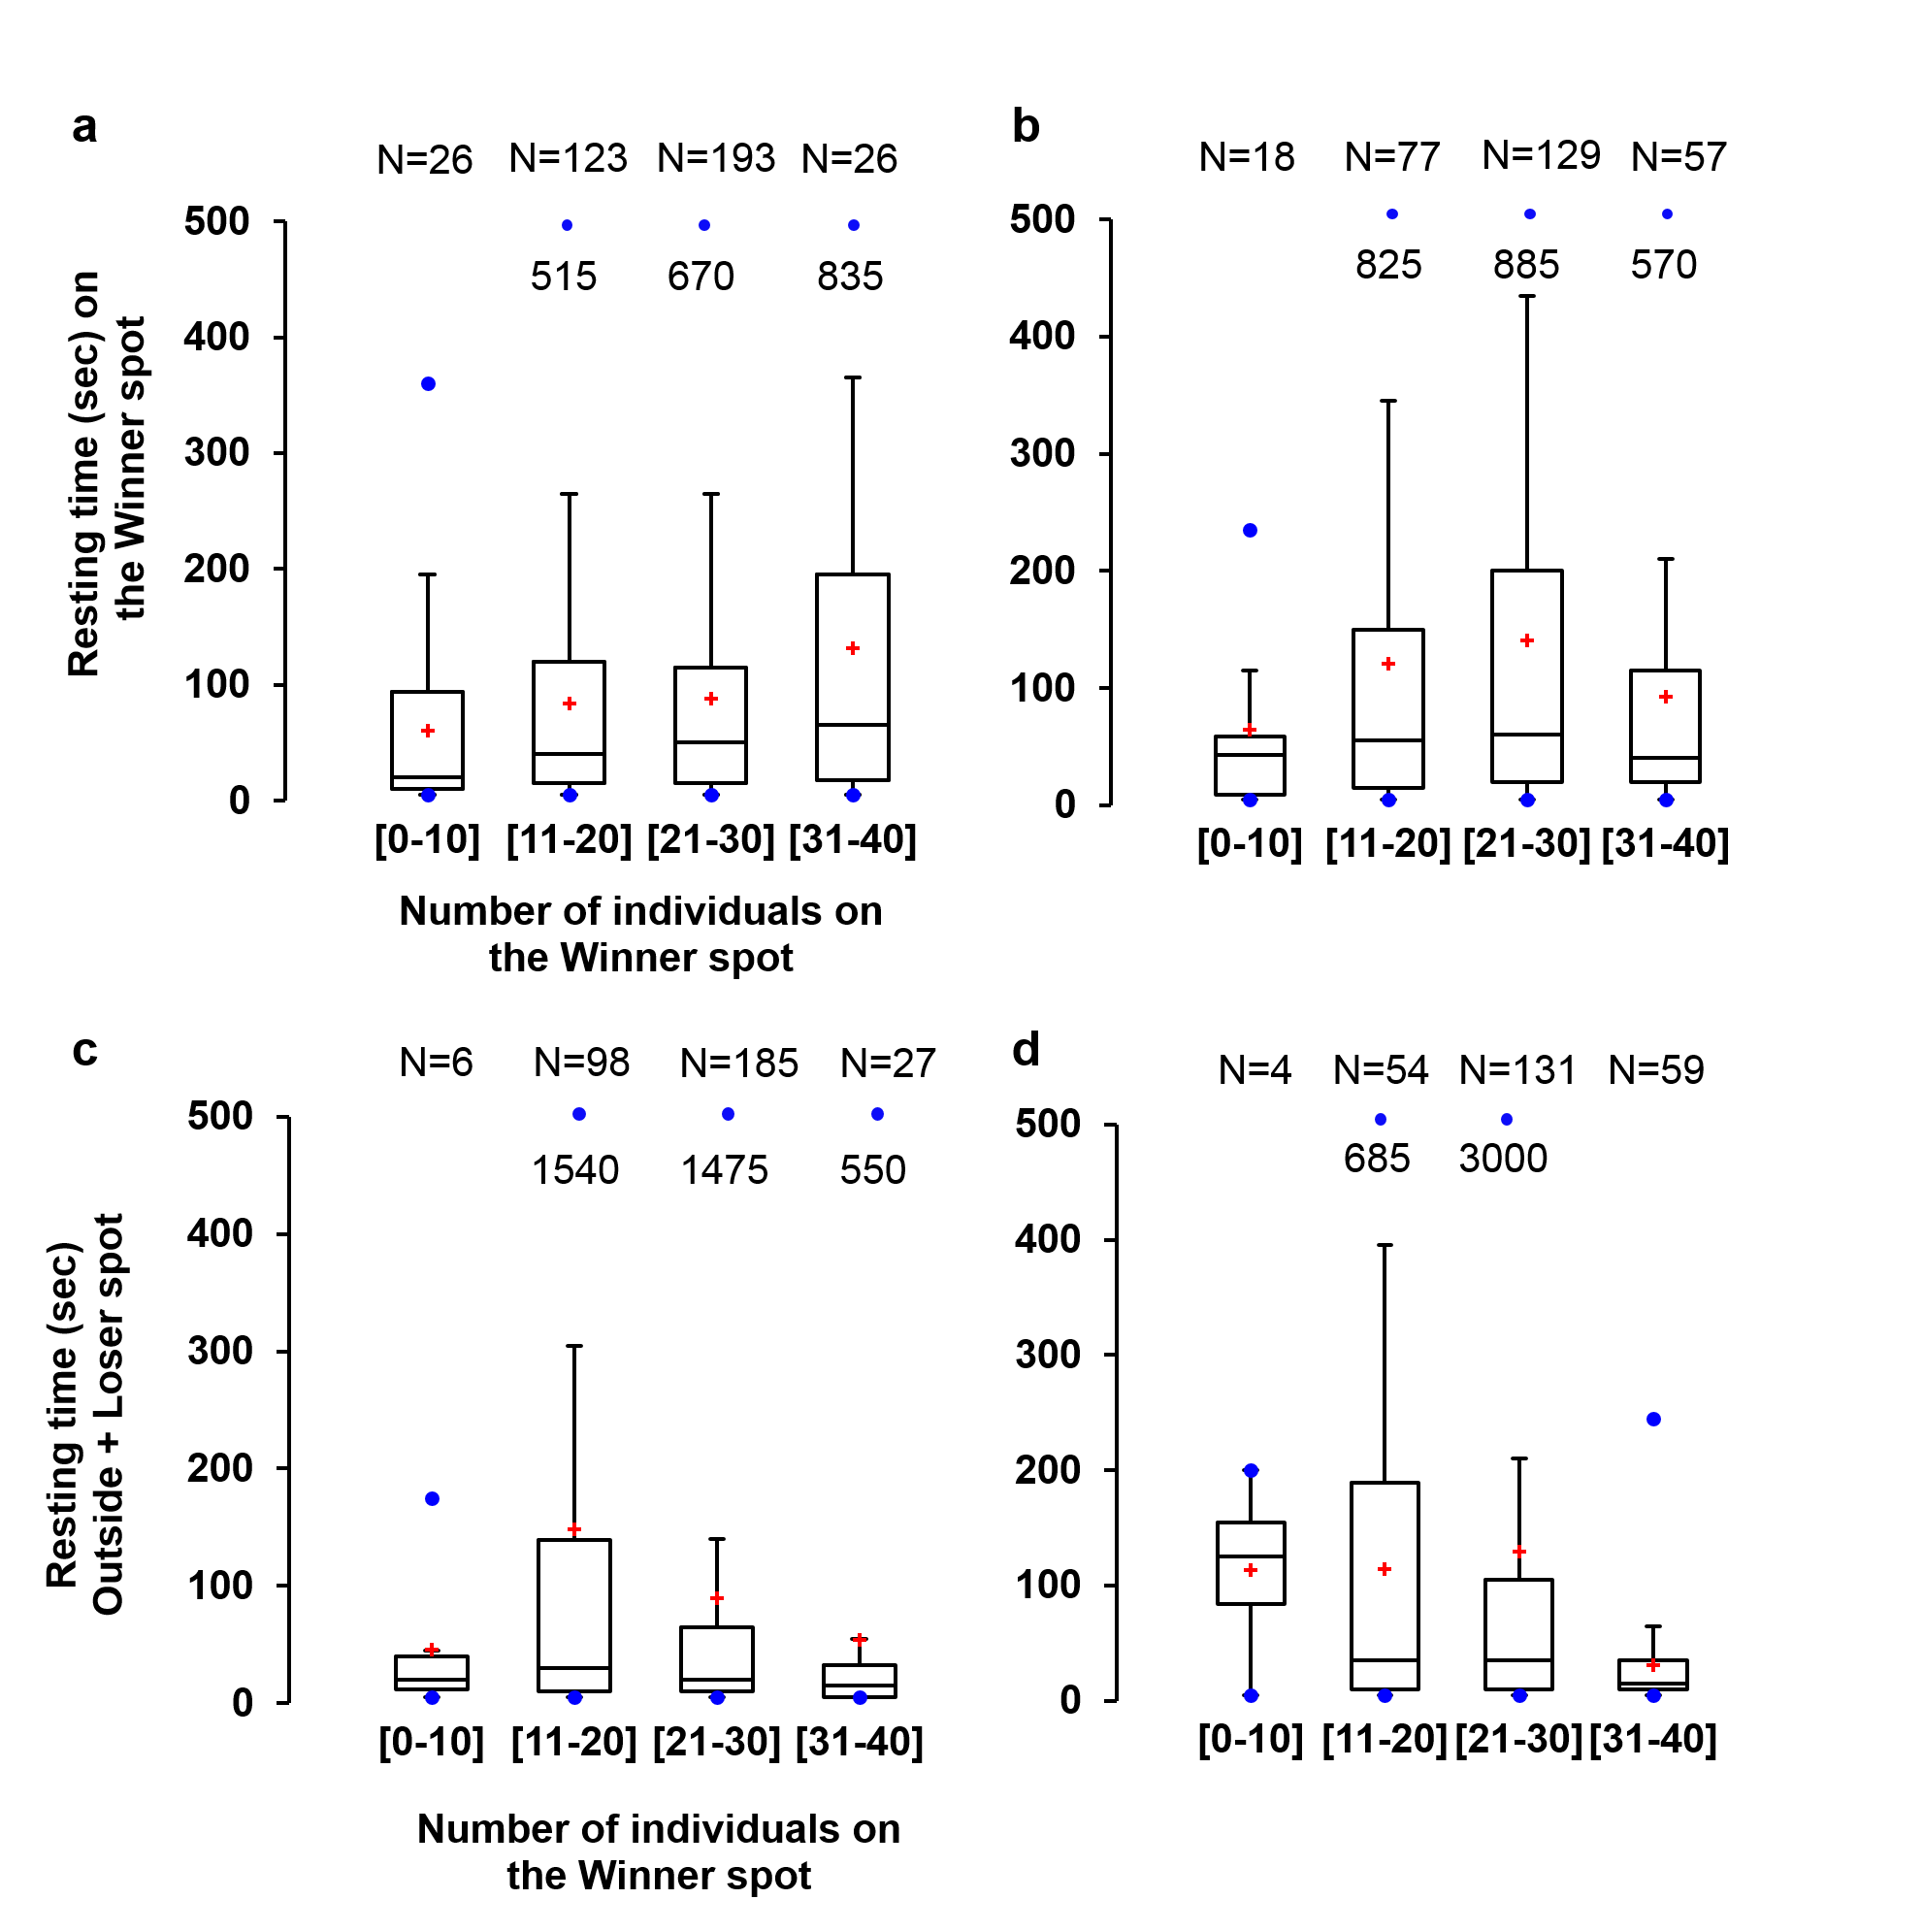
\includegraphics[width=1 \textwidth]{Figures/groupeffect.png}
		\rule{35em}{0.5pt}
		\caption[Groupeffect]{\textbf{Evidence of attractive and retentive effects of the group on individual larval behaviour.} Resting time (s) of tracked \textit{Lucilia sericata} larvae on the Winner spot (a) and Outside + Loser spot (c) as a function of the number of individuals on the Winner spot. Resting time (s) of tracked \textit{Calliphora vomitoria} larvae on the Winner spot (b) and Outside + Loser spot (d) as a function of the number of individuals on the Winner spot. For all boxplots, the first ten minutes were removed to reach a plateau regarding the accumulation of individuals on the Winner spot (Figure \ref{fig:choix}). No significant differences were observed in all boxplots according to the species (Kruskall-Wallis tests: 5a, KW=4.99, p=0.17; 5b, KW=4.77, p=0.17; 5c, KW=6.19, p=0.19; 5d (KW=13.73, p=0.003, Dunn’s test, p>0.05 for all multiple paired comparisons). The red crosses represent the means. N represents the number of elements. For trials in which aggregations were observed outside of either spot (\textit{L. sericata}, N=2; \textit{C. vomitoria}, N=4), the mean resting times of the individuals on the Winner spot were 75$\pm$112 s for \textit{L. sericata} and 17.9$\pm$13 s for \textit{C. vomitoria}. On the Loser spot, the corresponding times were 30$\pm$22 s for \textit{L. sericata} and 18.6$\pm$10 s for \textit{C. vomitoria}. The larvae spent less time on a spot when the number of individuals on the spot was low (means $\pm$SD throughout the experiment: Winner spot: \textit{L. sericata}: 6.8$\pm$3.5; \textit{C. vomitoria}: 2$\pm$1.5; Loser spot: \textit{L. sericata}: 3.7$\pm$4; \textit{C. vomitoria}: 2.4$\pm$2) (for comparison, see values in the text regarding trials yielding a collective choice for one spot).}
	\label{fig:groupeffect}
\end{figure}

\clearpage
%----------------------------------------------------------------------------------------
%	SECTION 5
%----------------------------------------------------------------------------------------
	\section{Discussion}
During the conspecific experiment, the majority of the larvae gathered on the food spots, and this distribution clearly differed from a random distribution (Figure \ref{fig:choix}). The collective choice of one spot, the Winner spot, out of the two spots occurred rapidly, within 5 min. The larval choice of one aggregation site is a consensus or collective decision \citep{deneubourg_dynamics_2002,conradt_consensus_2005}. The mechanisms underlying such collective decisions are self-organization and the use of local communication \cite{camazine_self-organization_2001}. Our individual tracking results showed that two mechanisms may be involved in this type of collective choice: the attraction and retention of the group (Figures \ref{fig:timenumb} and \ref{fig:groupeffect}). In blowfly larvae, this local communication likely involves a ground-marking signal that is passively left by crawling individuals; this larval signal has been shown to have an attractive/retentive effect on conspecifics \cite{boulay_evidence_2013}. The chemical profile of this cuticular signal has not yet been identified, but a recent study analysing the trail-following behaviour of blowfly larvae confirmed its existence \cite{boulay_first_2015}. Preliminary gas-chromatography results suggest that cholesterol could be one of the common signal for both species (Boulay, unpublished). According to the aggregation model presented by \citet{ame_collegial_2006}, it is likely that the larvae first explore the arena more or less at random but preferentially remain on food spots. Due to random asymmetry, the ground signal on one spot rapidly became stronger over time, which then created a Winner spot due to the progressive increase in the number of larvae on this spot. To support the hypothesis of the existence of this type of social amplification, simulation models, similar to those that have been used to investigate the self-organized collective decision-making process of cockroaches, will be constructed \cite{ame_collegial_2006}. The dynamics of aggregation was slower for the heterospecific group than for the conspecific group (Figure \ref{fig:choix}). Moreover, the mean number of individuals in the heterospecific group present outside the spots was greater than that found in the conspecific groups, whereas the mean number on the Winner spot was the same between the different groups, and the mean number on the Loser spot was lower in the heterospecific group (Figure \ref{fig:choix}). These results suggest the presence of a common retentive signal combined with a more species-specific attractive signal; moreover, these results suggest that the aggregation cues given by these two species are very similar and that at least one of the two species can detect and recognize the aggregation cues given by the other. However, a symmetric relationship in which the two species are able to recognize each other’s aggregation cues is possible.

In field conditions, various calliphorids larvae species are often observed in large aggregates composed of thousands of individuals of different instars and species. This strong aggregation behaviour is associated with an emerging property observed in large aggregates and commonly named the larval-mass effect \citep{charabidze_larval-mass_2011,slone_thermoregulation_2007}. The gathering of numerous larvae in dense masses can create a local increase in temperature that can reach 20\up{o}C above ambient. This modification of the thermal environment by larval groups decreases the duration of larval dependency on carrion (development time depends on temperature) and is considered one of the main benefits of gregarism in these species \cite{rivers_physiological_2011}. The cooperation observed between the two studied species is consistent with the Allee effect principle \cite{courchamp_allee_2008}. Aggregation behaviour allows larvae to reach a sufficiently large group size to receive benefits, such as heat generation and enzyme production \cite{rivers_physiological_2011}. Accordingly, heterospecific aggregation will allow larvae to reach this sufficient group size, particularly if the monospecific population is low. Such benefits can lead to an interspecific Allee effect. Our study highlights the importance of cooperative effects in blowfly larvae through the demonstration of active aggregation behaviour in conspecific and heterospecific groups. In natural conditions, full competition between larvae does not exist because each larval species has its own thermal preferences \cite{villet_contemporary_2010}. Conversely, segregation of two gathering species due to different thermal preferences has also been reported for closely related species \cite{villet_contemporary_2010}. Similar experiments should be conducted with more individuals, which will result in heat generation \cite{heaton_quantifying_2014}, and to study species segregation due to the specific thermal preferences of the larvae \cite{villet_contemporary_2010}. The notion of gregariousness often implies cooperation and/or competition. These two behaviours are the most fundamental principles that drive the evolution of social structures. The study of mixed-species groups offers biologists an interesting approach for exploring the frontiers between cooperation and competition in animal groups. Moreover, our results highlight that forensic entomologists should take into account the social behaviour of Diptera larvae, particularly the group size of larval masses, when estimating time of death.


	\section{Competing interests}
We have no competing interests.

	\section{Authors’ Contributions}
JB conceived of the study, design the study, collected data, carried out the statistical analyses, drafted the manuscript; DC conceived of the study, coordinated the study and helped draft the manuscript; VH gave final approval; JLD carried out the statistical analyses and helped draft the manuscript. All authors gave final approval for publication.   

	\section{Acknowledgments}
We thank the two anonymous reviewers for their very helpful comments. We thank F. Catteau for helping to track individuals. J.-L. Deneubourg is a Senior Research Associate from the F.R.S.-FNRS. 


%----------------------------------------------------------------------------------------
%	SECTION 6
%----------------------------------------------------------------------------------------
	\section{Supplementary materials}
    
\begin{figure}[h]
\centering
		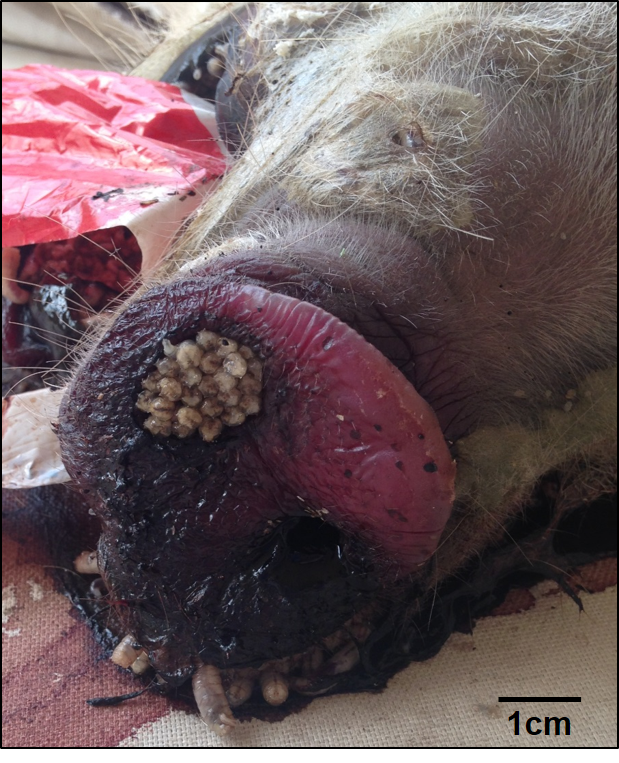
\includegraphics[width=0.5 \textwidth]{Figures/cochon.png}
		\rule{35em}{0.5pt}
		\caption[Cochon]{\textbf{Aggregation of necrophagous Diptera larvae on a pig cadaver (\textit{Sus scrofa}).} This aggregation was composed of Calliphoridae larvae and was located in a nostril (photo : J. Boulay).}
	\label{fig:cochon}
\end{figure}    

\begin{figure}[h]
\centering
		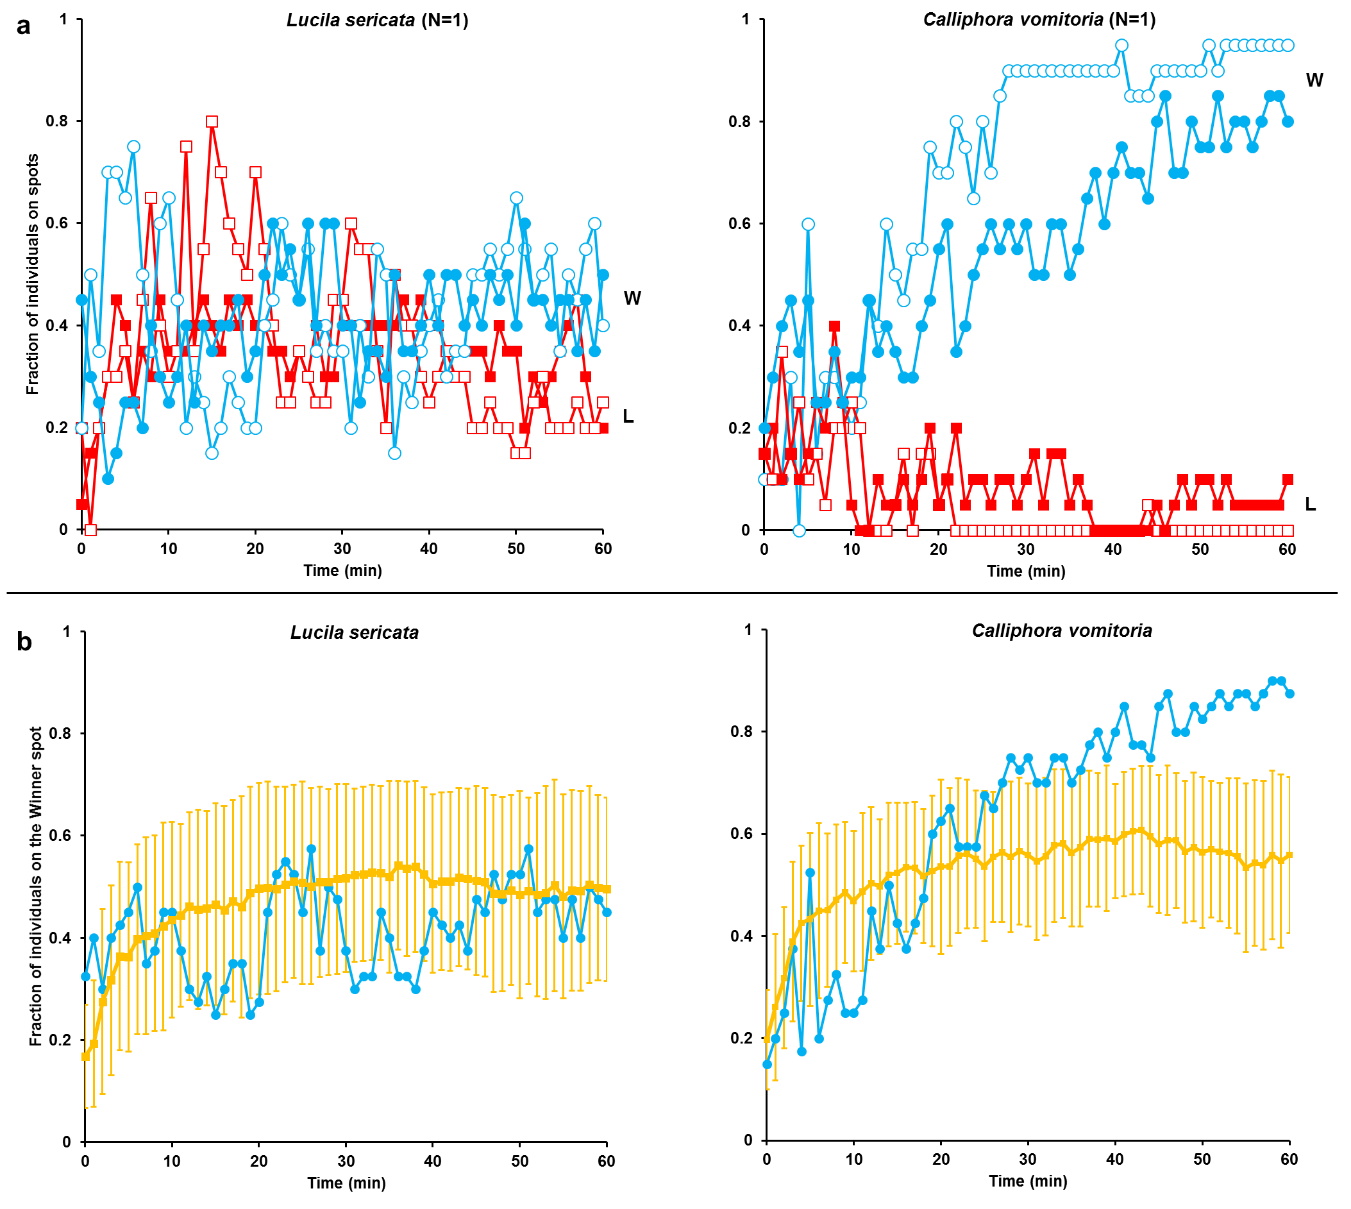
\includegraphics[width=1 \textwidth]{Figures/testagreg.png}
		\rule{35em}{0.5pt}
		\caption[Testagreg]{\textbf{Test of the effect of the marking technique on the aggregation of \textit{Lucilia sericata} and \textit{Calliphora vomitoria} larvae.} \textbf{a}, In this series of experiments, 20 larvae were marked using Lumicyano\up{TM} (filled dots) and 20 were not marked (white dots); an experiment was performed for each tested species, and collective choice for one spot was observed (Winner spot (W, blue lines); Loser spot (L, red lines)). For \textit{L. sericata}, the Winner spot sheltered 18 larvae, and the Loser spot had 9 individuals (binomial test: p=0.03). For \textit{C. vomitoria}, the Winner spot sheltered 35 individuals, and the Loser spot only had 2 (binomial test: p<0.0001). b, Fraction of individuals on the Winner spot during control experiments (in blue; sheltering marked and non-marked larvae) and during monospecific conditions (in orange; mean fraction ($\pm$SD) of non-marked individuals; seen in Figure \ref{fig:choix}). The marking method did not influence the aggregation dynamics of the intraspecific group composed by marked and non-marked conspecific individuals. Such results indicate that the marking technique used is non-invasive.}
	\label{fig:testagreg}
\end{figure}    

\clearpage

\textbf{Video S3. Collective choice of a \textit{Lucilia sericata} larvae group accelerated 20 times.} In green: the Winner spot; in red: the Loser spot. The focal individual was virtually marked by a white circle.

\textbf{Video S4. Collective choice of a \textit{Calliphora vomitoria} larvae group accelerated 20 times.} In green: the Winner spot; in red: the Loser spot. The focal individual was virtually marked by a white circle.

\textbf{Video S5. Collective choice of a heterospecific group accelerated 20 times.} Twenty \textit{Calliphora vomitoria} larvae were marked using the Lumicyano\up{o} and twenty \textit{Lucilia sericata} larvae were non-marked.
\\

\begin{figure}[h]
\centering
		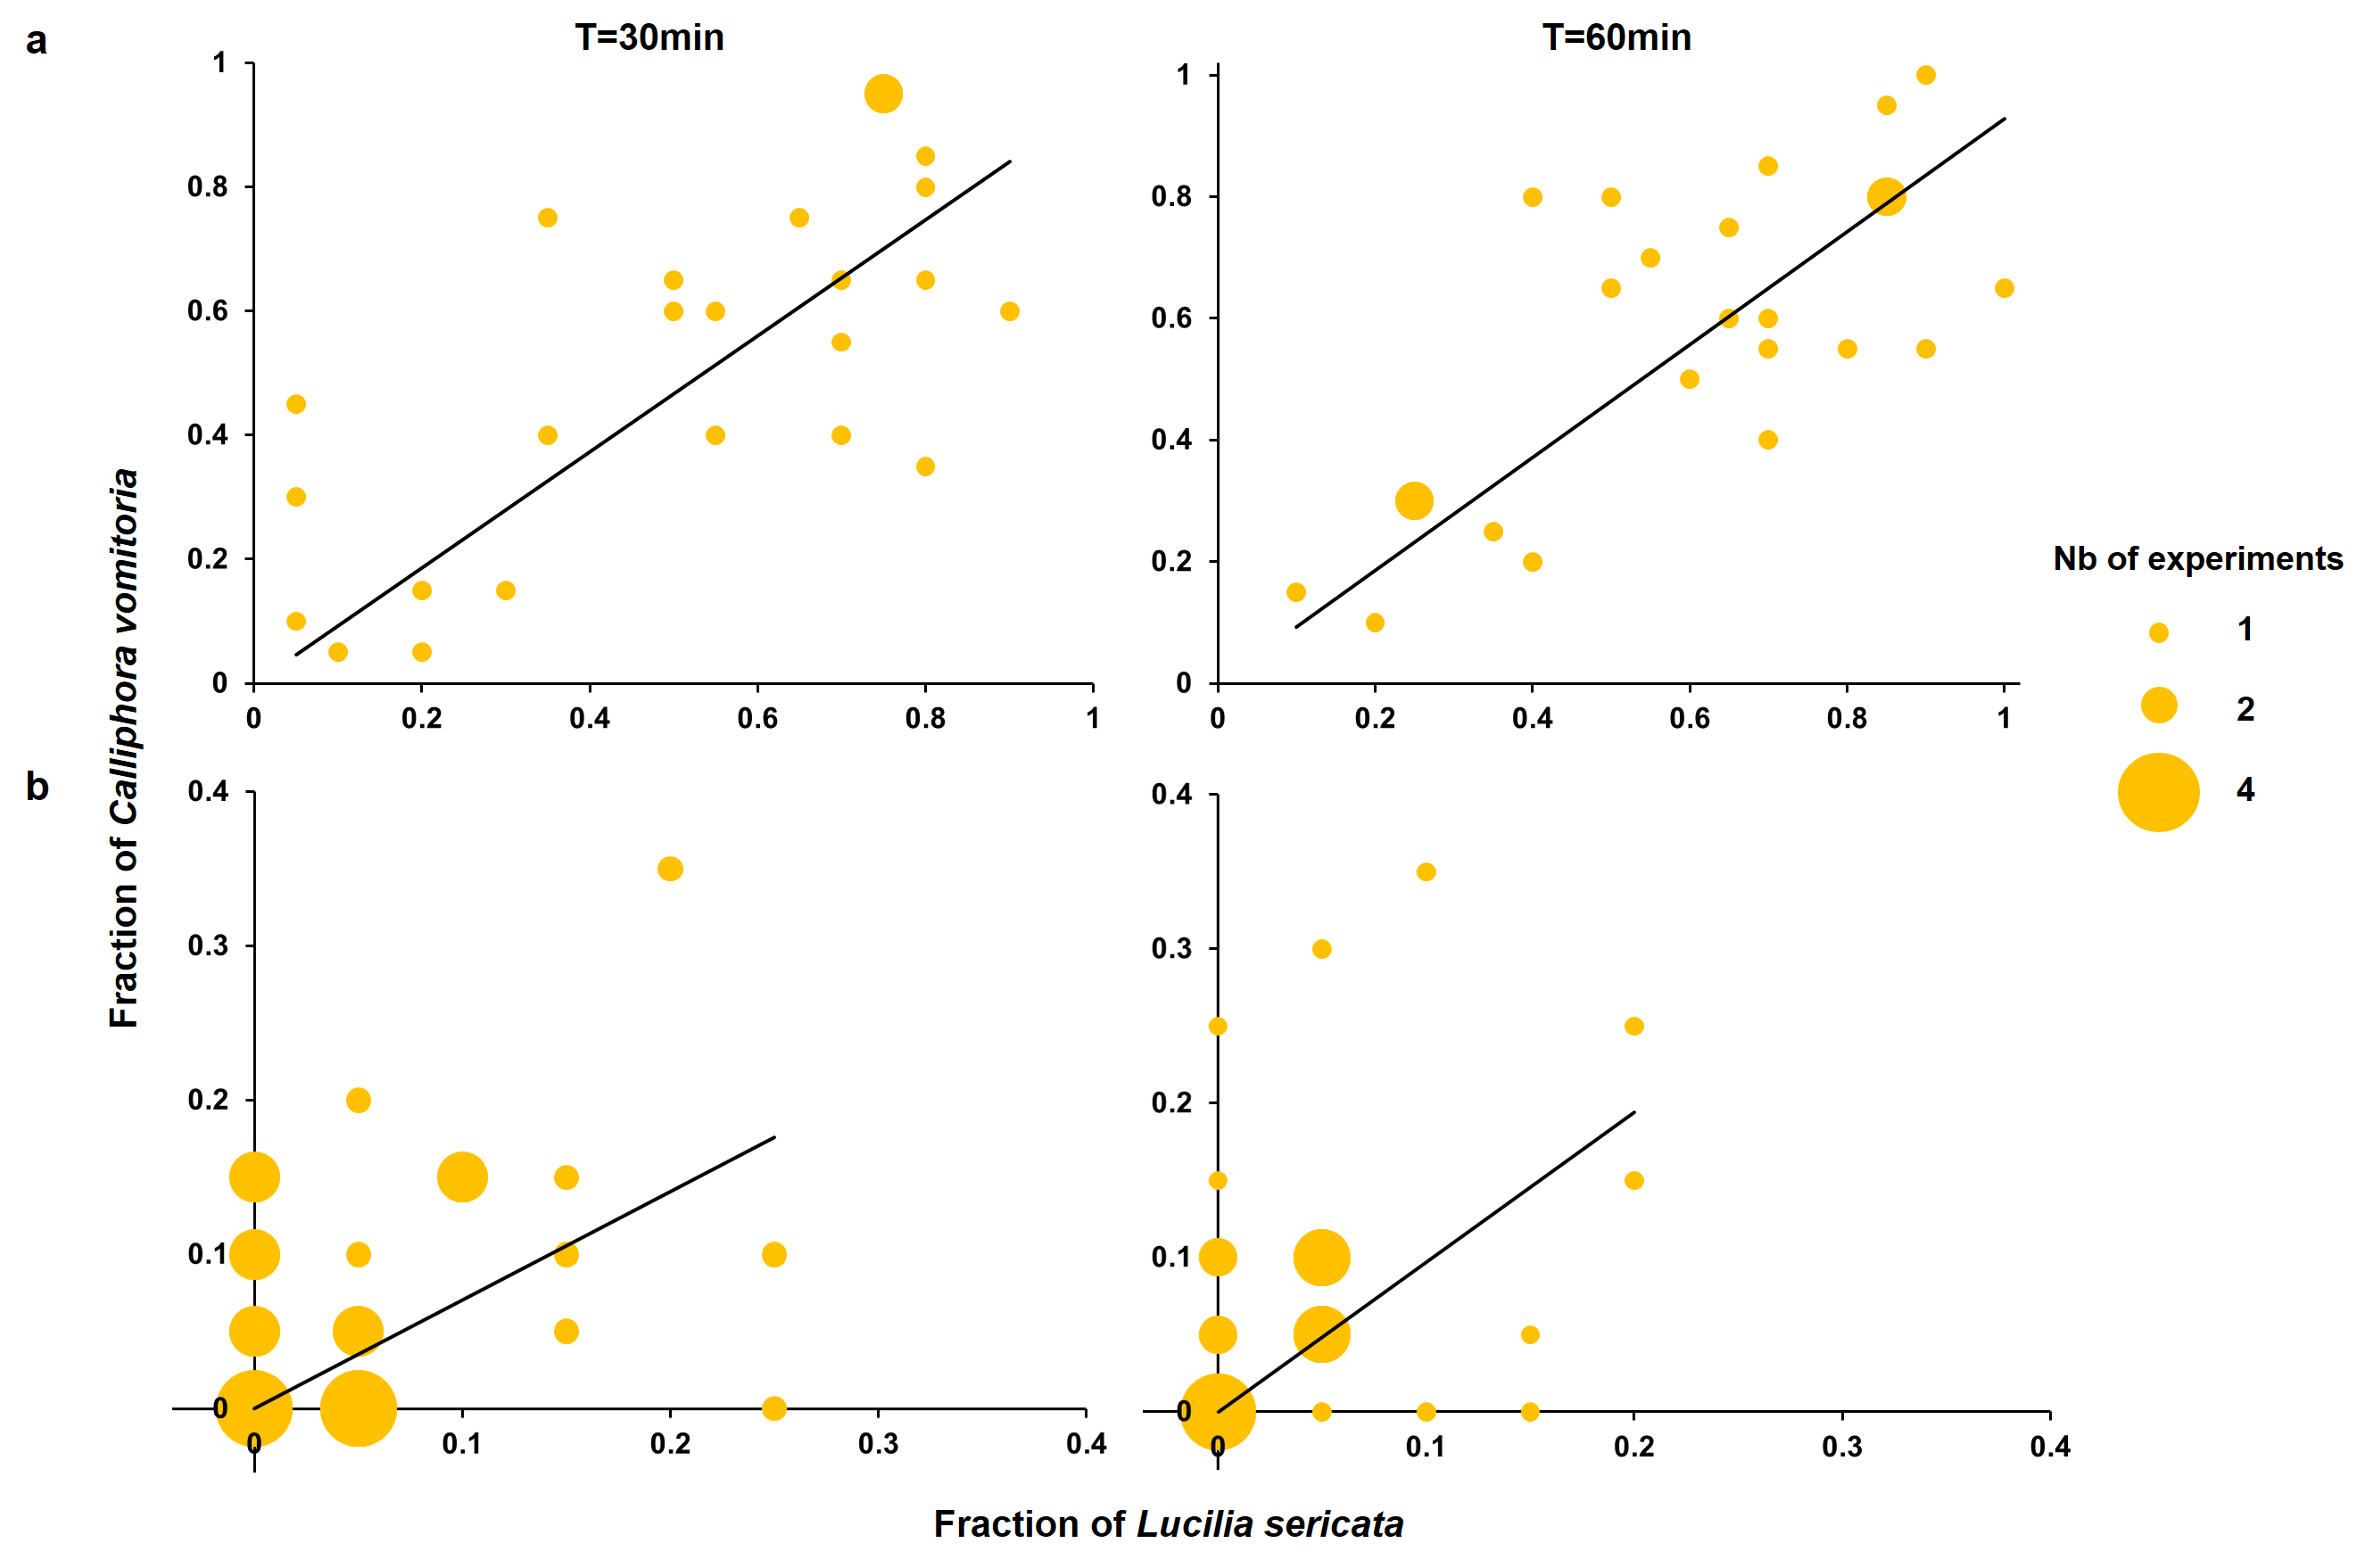
\includegraphics[width=1 \textwidth]{Figures/speciesvsspecies.png}
		\rule{35em}{0.5pt}
		\caption[Species]{\textbf{Repartition of the two studied species in heterospecific groups.} \textbf{a}, Fraction of individuals of each species on the Winner spot during the heterospecific condition experiment (N=24) at t=30 min (linear regression: R\up{2}=0.44; t=12.7, p<0.001) and t=60 min (R\up{2}=0.44; t=15.2, p<0.001). No differences were observed between the mean fractions of \textit{Lucilia sericata} and \textit{Calliphora vomitoria} at t=30 min (W=-26, p>0.5) and at t=60 min (W=50, p>0.1). \textbf{b} Fraction of individuals of each species on the Loser spot during the heterospecific condition experiment (N=24) at t=30 min (linear regression: R\up{2}=-0.1; t=4.3, p<0.001) and t=60 min (R\up{2}=-0.26; t=3.7, p<0.001). No differences were observed between the mean fractions of \textit{L. sericata} and \textit{C. vomitoria} at t=30 min (W=-58, p>0.1) and t=60 min (W=-66, p>0.1).}
	\label{fig:species}
\end{figure}    

\begin{landscape}
\begin{table}[t]
	\caption[Transition]{\textbf{Transitions of tracked individuals between spots during conspecific experiments.} In this study, transition is defined as the duration of time between a zone exit (e.g., Winner spot or Loser spot) and re-entry into that same zone. For both species, the mean number of transitions from Winner to Winner was significantly higher than that obtained for the other transition types (Dunn’s tests, $\alpha$=0.025, p<0.001). For \textit{L. sericata}, no differences were observed in the mean transition times between Winner-to-Winner and Loser-to-Loser transitions (KW= 18.21, p=0.0004; Dunn’s tests, $\alpha$=0.025, p>0.05) and between Winner-to-Loser and Loser-to-Winner transitions (Dunn’s test, $\alpha$=0.025, p>0.05). In contrast, for \textit{C. vomitoria}, the mean transition time for Winner-to-Winner transitions was significantly higher than that for Loser-to-Loser transitions (KW= 24.49, p<0.0001; Dunn’s test, $\alpha$=0.025, p<0.01). No difference was observed between the mean Winner-to-Loser and Loser-to-Winner transition times (Dunn’s test, $\alpha$=0.025, p>0.05).}
    \centering
	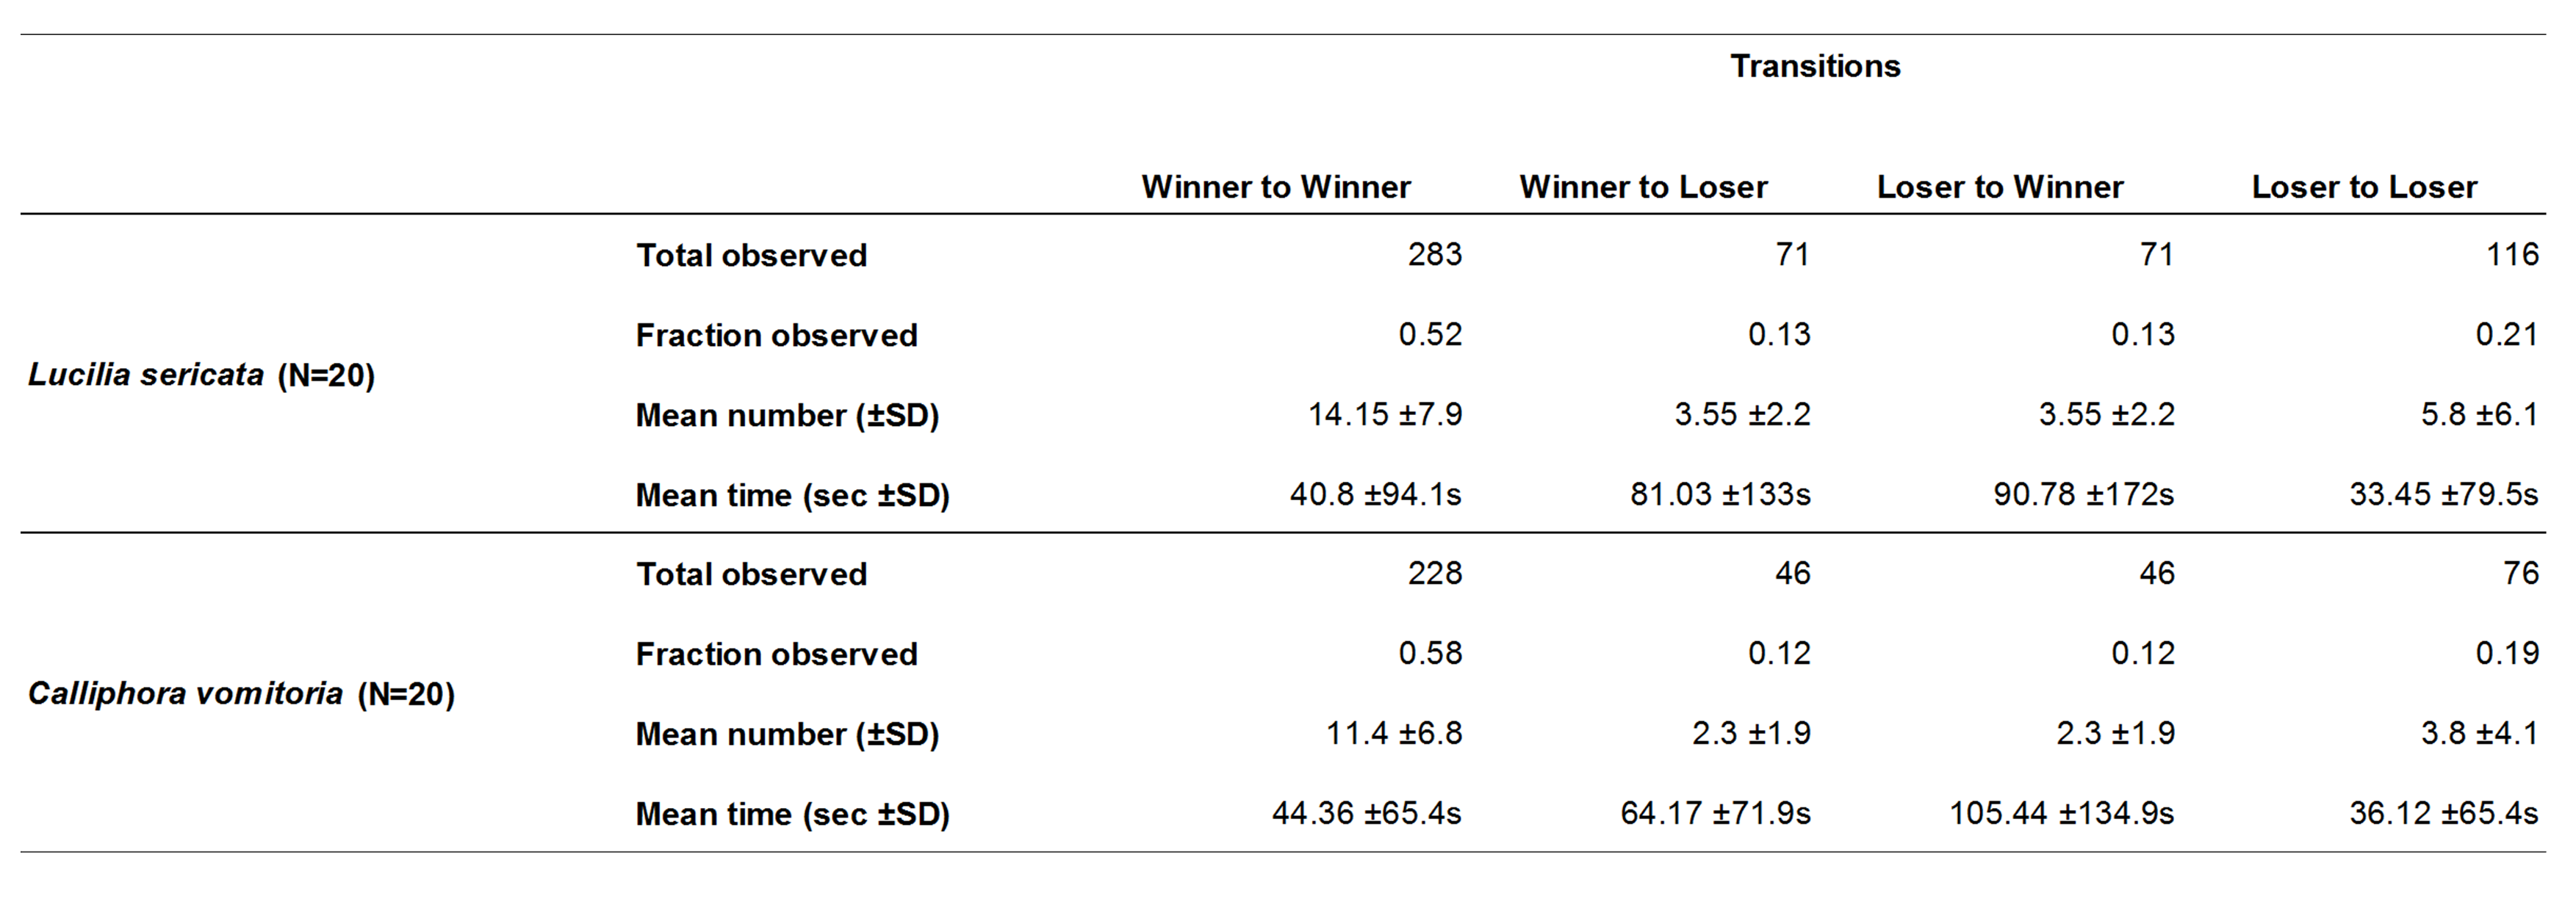
\includegraphics[width=1.5 \textwidth]{Figures/table2.png}
		\label{tab:transition}
\end{table}
\end{landscape}    

\clearpage    
    
    
    
    
    
    
    
    
    
    
